\section{Hard- und Software}
Zur Integration eines hochschulweiten Informationsmanagements können bezüglich der IT mehrere Ansätze gefahren werden.

Zum einen kann eine ganzheitliche integrierte Lösung verwendet werden. Die Universität Hamburg hat einen vollständigen Neuanfang bezüglich der Campussoftware gewagt mit der integrierten Gesamtlösung „CampusNet“ der Datenlotsen Informationssysteme GmbH. Die Entscheidung dazu resultierte aus der Zusammenlegung mehrerer Fachbereiche mit sehr unterschiedlichen Teillösungen zu einzelnen Fakultäten. Die verschiedenen Teillösungen waren größtenteils inkompatibel oder aufgrund von Eigenentwicklung schwer wartbar.\footnote{\cite{dini_webportale_2007}}

Laut Günter Müller, Leiter des Rechenzentrums, existieren an der Hochschule Emden Leer derart verschiedene Teillösungen nicht. Auch würden sich Eigenentwicklungen auf vernachlässigbare Systeme beschränken. Software würde grundsätzlich für die gesamte Hochschule eingesetzt.\footnote{Interview}

Der Einsatz einer integrierten Gesamtlösung zur Beseitigung von Inkompatibilitäten und schwer wartbaren Eigenentwicklungen kann somit keine Argumentationsgrundlage sein.
Des Weiteren reicht die in dieser Ausarbeitung getätigte Analyse des Ist-Zustands und der Anforderungen nicht aus, um einen vollständigen Anforderungskatalog zu bilden, auf dessen Grundlage eine integrierte Gesamtlösung gefunden werden kann.

Stattdessen wird auf eine flexible Lösung gesetzt, welche den Einsatz einzelner Fachanwendungen zur Lösung bestimmter Probleme vorsieht. Personelle und finanzielle Ressourcen sind dadurch flexibler einsetzbar, auf veränderte Anforderungen an eine Lösung kann flexibler reagiert werden und die Abhängigkeit von einem Anbieter für alle Anwendungen wird aufgelöst.

\subsection{Kernanforderungen}
Bei Core-Systemen wird weiterhin auf Appliance Lösungen gesetzt. Das minimiert Fehlerpotenzial und den operativen Betrieb.\footnote{Interview}

Softwaresysteme laufen auf virtuellen Maschinen. Die bessere Hardwareauslastung und Möglichkeit der automatisierten Administration kann finanzielle und personelle Ressourcen sparen.\footnote{\cite{baun_servervirtualisierung_2009}}

Die Systeme sind weniger abhängig von der Hardware, was dessen Austausch erleichtert. Netzwerkanbindung, Rechenleistung und Speicherkapazität sind somit flexibler an sich verändernde Anforderungen anpassbar.

Die eingesetzte Software soll in die Systemlandschaft integrierbar, lösungsorientiert und möglichst barrierefrei sein, sowie möglichst unabhängig von Client-seitig eingesetzten Systemen. Letzteres unterstützt auch den Ansatz der Freiheit in Forschung und Lehre.

Die Systemunabhängigkeit kann durch Webanwendungen im Sinne des Ansatzes Software as a Service (SaaS) erreicht werden. Um möglichst alle gängigen Browser und Endgeräte zu unterstützen, sollten die Anwendungen den Standards des World Wide Web Consortiums (W3C) und, soweit möglich, dem Ansatz responsive design gerecht werden. Dadurch kann auch dem Trend bring your own device Rechnung getragen werden.

\subsection{Bereichsübergreifende Basissysteme}
In den Bereichen Forschung, Lehre und Verwaltung fallen informationstechnologische Aufgaben an, für die eine zentrale IT-gestützte Lösung geschaffen werden kann. Das verringert redundante Daten und Systeme sowie administrative Aufwände. Im folgenden werden Lösungen für einzelne Aspekte des Informationsmanagements aus IT-Sicht vorgestellt, die in allen drei Bereichen genutzt werden können. Weiterhin dienen sie teilweise als Grundlage für spezialisierte Systeme.

\subsubsection{Identity Management}
Um die Anzahl an verschiedenen Accounts zu minimieren, sollten die Benutzer zentral gepflegt werden. Dies kann in einem Verzeichnisdienst wie dem bereits eingeführten Active Directory geschehen. Die Authentifizierung an einem System findet dann nicht am System selbst statt, sondern mit Hilfe des Verzeichnisdienstes. Der Anwender muss sich nur einen Anmeldenamen zzgl. Kennwort merken, um sich an den verschiedenen Systemen anzumelden. Weiterhin gilt eine Aktualisierung von Informationen global, wodurch Inkonsistenzen aufgelöst werden.

Davon ausgenommen dürfen Systeme sein, deren spezielle Sicherheitsanforderungen nicht mit diesem Konzept vereinbar wären.

In allen anderen Fällen ist zuzüglich zum zentralen Verzeichnisdienst auch ein SingleSignOn (SSO) Mechanismus empfehlenswert\footnote{\cite{zahn_itmanagement}}, wie es an der Universität Augsburg durch das System Webauth umgesetzt ist.

Die sich im Einsatz befindlichen Websysteme sollen auf SSO umgestellt werden, um dem Benutzer eine möglichst integrierte Landschaft zu bieten. Weiterhin sollte jedes System aus Sicherheitsgründen insofern angepasst werden, dass auch ein SingleSignOff möglich ist. Die zentrale Abmeldung soll gewährleisten, dass die Benutzenden auf allen Systemen, auf denen sie sich bewegt haben, mit einem Klick abgemeldet sind.

Die Benutzerdatenpflege sollte auf den einzelnen Systemen ausgeschaltet sein und ausschließlich über ein zentrales Formular geschehen. So wird ein konsistenter Datenbestand gesichert. Insofern die Informationen in anderen Systemen benötigt werden, müssen diese vom zentralen System direkt angefordert oder, wenn die Daten im System persistiert sein müssen, automatisiert und über gesicherte Verbindungen verteilt werden. Ein weiterer Vorteil ist, dass die Informationen, da zentral gesammelt, auch zentral ausgewertet werden können.

Diese zentrale Informationsbasis ermöglicht zentrale persönlichen Informationen mit Informationen anderer Art aus anderen Systemen anzureichern und weiterzuverwenden. So können automatisierte Reports über Forschungsprojekte erstellt werden, Expertisen zu bestimmten Themen identifiziert werden oder für die Verwaltung Verknüpfungen von Personen zu verwaltungstechnischen Aufgaben wie zum Beispiel Exmatrikulation. Die Umsetzung ist dabei individuell an die Gegebenheiten und Informationsbedarfe der Hochschule anzupassen.\footnote{\cite{vogl_fortschritte_2012}} Aus diesem Grund wird die technische Lösung eine Individuallösung werden.

\subsubsection{Geschäftsprozesse}
Neben der Forschung gibt es an Hochschulen gerade im Verwaltungsbereich viele Geschäftsprozesse, die in der Regel immer gleich ablaufen. Problem ist, dass Personen unterschiedlichster Bereiche involviert sind und die Prozesse nicht ausreichend definiert sind.\footnote{\cite{becker_prozesse_2010}}

Hier empfiehlt sich der Einsatz von Business Process Management. Nach dem Identifizieren möglicher Prozesse werden diese modelliert, konkretisiert und zuletzt digitalisiert.

Die Modellierung der Prozesse im ersten Schritt sollte auf abstraktem Niveau stattfinden. Dies erleichtert den Einstieg und macht Verbesserungspotenziale sichtbarer. In der WWU Münster wurde dafür die PICTURE Methode verwendet.
Im zweiten Schritt kann der ggf. angepasste Prozess konkretisiert und in Form des Industriestandards Business Process Model Notation (BPMN) digital notiert werden. Ein Client-Tool zur Erstellung von BPMN ist das Activiti BPMN 2.0 Eclipse Plugin.\footnote{\url{http://docs.codehaus.org/display/ACT/Activiti+BPMN+2.0+Eclipse+Plugin}}

Mit Hilfe der zentralen Business Process Management (BPM) Platform activiti können die Prozesse aktiv den Workflow verbessern, Konsistenz wahren und zeitliche Ressourcen sparen.  Die Plattform ermöglicht REST Anfragen, wodurch die Prozessinformationen auch in andere Applikation integriert werden können. Der Activiti Explorer ermöglicht den voll funktionalen Zugriff via Weboberfläche. Somit wird der Kernanforderung SaaS Rechnung getragen. Weiterhin ist Activiti Open Source und somit ausbau- und anpassungsfähig.\footnote{\url{http://activiti.org/index.html}}

Durch activiti wird es möglich sein die Automatisierung von einzelnen Prozessen Stück für Stück voranzutreiben indem manuelle Aufgaben gegen Automatismen ersetzt werden. Einzelne Teile des Workflows können dann automatisiert Scripte starten, E-Mails verschicken und ähnliches und somit stückweise die manuelle Bearbeitung reduzieren. Außerdem können Serviceanfragen mit diesem Tool zentralisiert verwaltet werden. Durch Definition von Pflichtfeldern für einzelne Prozessschritte können vorab benötigte Informationen festgelegt werden, sodass Nachfragen vermieden werden.

\subsubsection{Content Management}
Um den wachsenden Anforderungen in Bezug auf Content Management genüge zu tun wurde an der WWU Münster das Enterprise Content Management System alfresco eingeführt. Auch an einer kleinen Hochschule kann ein solches System eingesetzt werden. Alfresco bietet diverse Vorteile. Die für dieses Konzept Relevanten werden hier kurz aufgelistet:\footnote{\cite{kloetgen_2012}}

\begin{itemize}
	\item Unterstützung für mobile Endgeräte
	\item Anpassungs- und ausbaufähig
	\item diverse Zugriffsmöglichkeiten zur Nutzung innerhalb bekannter Standardanwendungen
	\item Publikation in sozialen Netzwerken
	\item Unterstützung verschiedener Standardschnittstellen
	\item Activiti Workflow Engine
	\item Metadaten
\end{itemize}

Alfresco bietet damit die ideale Grundlage verschiedenste Informationen zu verwalten sowie die Unterstützung des vollständigen Dokumenten-Lifecycles - von der Erstellung über die Bereitstellung bis zur Archivierung. 

Die Art des Zugriffs auf Dokumente ist dynamisch dank der Unterstützung zahlreicher Standards. Somit kann die Integration der Dokumente angepasst an die jeweiligen Anforderungen geschehen. Ein Dokument, welches an verschiedenen Orten auf verschiedene Arten bereitgestellt werden soll, kann dank Alfresco zentral aktualisiert werden und an allen Zugriffsstellen die aktuellste Version bereitgestellt wird.

Dennoch ist das System flexibel genug auch bestimmte Versionen eines Dokuments bereitzustellen. Dank der integrierten Versionierung entfällt außerdem der aufwendige Wiederherstellungsprozess. Durch die Möglichkeit Metadaten anzugeben, wird der Weg für eine brauchbare Dokumentensuche geebnet.

\subsection{Spezialsysteme}
Unter Spezialsystemen sind hier Softwarelösungen zu verstehen, die bei speziellen Aufgaben im Hochschulalltag unterstützen sollen.

\subsubsection{Verwaltungssoftware}
Software, die speziell in der Verwaltung genutzt wird, ist in dieser Ausarbeitung ausgenommen, da die Anforderungen sehr speziell sein können und die Wissensbasis innerhalb dieser Ausarbeitung um die Anforderungen der Hochschule an eine solche Software nicht ausreicht, um eine Empfehlung zu geben.

Erwähnt werden sollte dennoch, dass die Universität Karlsruhe erfolgreich Schnittstellen zu den HIS-Systemen integriert hat.\footnote{\cite{dini_webportale_2007}}

Da das Konzept dieser Ausarbeitung für die Hochschule Emden-Leer auf einem ähnlich flexiblen Ansatz basiert, wie der bereits umgesetzte Ansatz der Universität Karlsruhe, besteht die Möglichkeit, dass auch Verwaltungssoftware integriert werden kann, insofern diese die genannten Kernanforderungen erfüllt.

\subsubsection{Lernplattform}
Die Hochschule setzt bereits erfolgreich und in vielen Bereichen das System moodle ein. Die Nutzung der Funktionen variiert dabei zwischen den einzelnen Fachbereichen.
Solange moodle die Anforderungen der Hochschule an eine Lernplattform erfüllt, besteht kein Grund das System auszutauschen.

Neben den bereits genutzten Standardfunktionen ist moodle ausbaufähig.

Beim Aufruf von moodle soll die Authentifizierung durch einen SSO Mechanismus geschehen. Hat sich ein Benutzer bereits an einem anderen System authentifiziert, ist dieser beim Aufruf sofort angemeldet. Für das Lernraumsystem moodle gibt es bereits ein SSO Plugin.\footnote{\url{http://sourceforge.net/projects/moodleldapsso}} Integriert werden sollte auch der SingleSignOff Mechanismus.
Statt der Stammdatenänderung via moodle wird der entsprechende Menüpunkt ausgeblendet oder auf ein zentrales Formular weitergeleiten, um persönliche Informationen zentral und damit konsistent zu halten.

Die in den Kursen zur Verfügung gestellten Dateien jeglicher Art werden in alfresco gepflegt und von moodle angebunden. Die entsprechenden Schnittstellen und Plugins müssen nicht neu entwickelt werden.

Vorteil ist, dass die Dokumente in alfresco verwaltet werden. In moodle kann dann eine bestimmte Version oder die jeweils aktuellste referenziert werden. Bei den Dokumenten kann es sich um Textdokumente, Audio- oder auch Videodateien handeln. Durch alfrescos Unterstützung für mobile Endgeräte außerdem den Zugreifenden auch die Möglichkeit gegeben ein Dokument auf den verschiedensten Endgeräten anzuzeigen bzw. wiederzugeben.

Dank alfresco können Dokumente nicht nur innerhalb moodle via Weboberfläche aufgerufen werden, sondern auch bequem via Filesystem. Eine Datei kann somit auf verschiedene Art und Weise abgerufen werden – je nach dem welchen Weg der Anwender für den aktuell praktikabelsten hält.

\subsubsection{Publikationen}
Um Wissenschaftler bei der Publikation von Zeitschriften zu unterstützen, kann die Plattform Open Journal System (OJS) eingesetzt werden, wie es auch in der WWU Münster getan wird. Es bietet die Möglichkeit elektronische Zeitschriften zu verwalten und den gesamten Publikationsworkflow abzubilden.\footnote{\cite{kloetgen_2012}}

Grundsätzlich sollte auch ein Workflow in activiti implementiert werden, der bei der Publikation unterstützt. So können wichtige Metadaten aufgenommen und an relevante Systeme weitergegeben werden. Ändern sich Systeme oder kommen neue hinzu, müssen sich Wissenschaftler nicht umgewöhnen, sondern nutzen weiterhin den in activiti hinterlegten, für die neuen Systeme jedoch angepassten, Prozess. Dadurch besteht auch die Möglichkeit ein publiziertes Dokument zusätzlich in alfresco abzulegen, wenn ein Anwendungsfall dies benötigt.
OJS bietet die Möglichkeit der Authentifizierung via Single Sign On. Dies geschieht via Shibboleth.\footnote{\url{https://pkp.sfu.ca/wiki/index.php?title=Setting_up_authentication}}

Neben der Konfiguration von Single Sign On sollte auch hier den Benutzenden die Möglichkeit des Single Sign Off gegeben werden.

\subsubsection{Evaluation}
Wie auch die Universität Münster\footnote{\url{https://www.wiwi.uni-muenster.de/fakultaet/de/studium/lehrevaluation}} und die TU Dortmund\footnote{\url{https://www.itmc.uni-dortmund.de/dienste/e-learning/umfragewerkzeuge.html}} setzt die Hochschule Emden Leer bereits die Software EvaSys zu Evaluationszwecken ein. Sie ist webbasiert und entspricht damit dem Software as a Service Gedanken.
Seit Version 5 unterstützt EvaSys auch die SingleSignOn Authentifizierung\footnote{\url{http://www.ku.de/fileadmin/190304/Feature_Function_Benefit_EvaSys_V5.0_DE.pdf}}, welche auch an der Hochschule Emden Leer eingesetzt werden soll.

\subsubsection{Campus Portal}
Ein Campus Portal dient als zentrale Anlaufstelle für alle Hochschulangehörigen und ist ein personalisiertes Webportal. Es soll die Verwaltung persönlicher Daten ermöglichen, eine Übersicht über informationstechnische Funktionen inklusive Weiterleitung zum entsprechenden System integrieren, sowie aktuell relevante Informationen in Form einer Agenda anzeigen. Das Campus Portal soll also als Startpunkt dienen.

Unter dem Begriff informationstechnischer Funktionen sind hier alle Werkzeuge und Spezialsysteme(siehe oben) zu verstehen, die einem bestimmten Zweck dienen. Eine Selbstimplementierung für die bereitzustellenden Funktionen soll dabei vermieden werden.

Stattdessen soll, wie in den Kernanforderungen aufgenommen, auf existierende Systeme gesetzt werden, sofern dies möglich ist. Die Kernanforderungen an solche Systeme, nämlich integrierbar und systemabhängig (SaaS) zu sein, wird nun deutlich, da solche Systeme im Campus Portal integriert werden sollen.

Ein solches Campus Portal ist vor allem der Informationsübersicht dienlich. Durch personalisierte und dynamisch generierte Inhalte gewinnen die Benutzenden einen Überblick über die Informationen, die sonst in verschiedenen Systemen verteilt sind. Der Aufbau eines Campus Portals und die Integration der Spezialsysteme kann schrittweise erfolgen, sollte jedoch zur Akzeptanzgewinnung bei Veröffentlichung eine gewisse Menge externer Systeme integrieren.

Die Universität Karlsruhe hat im ersten Schritt das Veranstaltungsmanagement und die Prüfungsverwaltung der Software-Systeme der HIS GmbH in das Portal integriert.

Orientiert am Anforderungskatalog der WWU Münster an ein solches Portal und unter der Voraussetzung, dass die in diesem Konzept genannten Systeme umgesetzt werden, kann ein zukünftiges CampusPortal folgende Informationen konsolidieren:

\begin{itemize}
	\item Kalender
	\begin{itemize}
		\item Abonnement-Prinzip
		\item inklusive Detailinformationen, zum Beispiel Kontoinformationen für Rückmeldegebühren
		\item Agenda aus moodle
	\end{itemize}
	\item Referenz zu gewählten Kursen (moodle)
	\item Referenz zum E-Mail-Portal (Outlook Web App)
	\item Suchmaschine
	\item offene Tasks im BPM System
	\item Start möglicher Tasks im BPM System (zum Beispiel Workflow für die Publikation)
	\item offene Evaluationen
\end{itemize}

Neben den in diesem Konzept genannten Systemen, könnten weitere Spezialsysteme in das Campus Portal integriert werden. Der Anforderungskatalog der WWU Münster enthält außerdem:

\begin{itemize}
	\item Stundenplan
	\item Vorlesungsverzeichnis inkl. Details
	\item Leistungsübersicht
	\item Hochschulleben
	\begin{itemize}
		\item Mensapläne
		\item Hochschulsport
		\item Veranstaltungen
	\end{itemize}
	\item Einführung in die Benutzung
\end{itemize}

Alternativ zur Einführung in die Benutzung kann auch das Konzept eines Hilfesystems integriert werden, das via Sprechblasen Hilfestellungen oder Erläuterungen anzeigt zur jener Funktion, auf der sich der Mauszeiger gerade befindet.

Die technische Struktur kann analog zu der des Portals myWWU der Universität Münster aufgebaut sein, wie im Folgenden abgebildet.
\begin{figure}[h!]
	\centering
	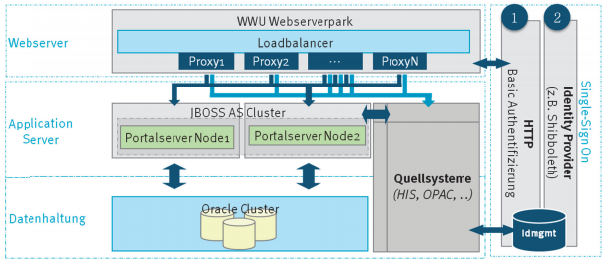
\includegraphics[width=\textwidth]{kapitel/gruppe3/bilder/struktur_mywwu}
	\caption{technische Struktur des Portals myWWU der Universität Münster}
	\label{fig_struktur_mywwu}
\end{figure}
\newpage

\subsubsection{Integrierte Gesamtsuche}
Wissenschaftliche Informationen sind häufig in verschiedenen Systemen angesiedelt. 
Durch die Einführung eines Systems zur integrierten Gesamtsuche würde die Suche 
an zentraler Stelle ausgeführt. Einzelne Systeme werden beim Suchen nicht vergessen 
und die Integration neuer Systeme als Informationsbasis des wissenschaftlichen 
Umfelds wird dauerhaft kommuniziert statt einmalig, wie es beispielsweise beim 
Versand einer Info-E-Mail der Fall wäre.

Die WWU Münster nutzt dafür einen „Suchmaschinen-basierte[n] Ansatz auf Basis der Software Primo von der Firma Ex Libris“.\footnote{\cite{vogl_fortschritte_2012}} Dafür nötig ist eine Normalisierung der Datenformate interner und externer Quellen, welche „insbesondere auf der Detailebene […] aufwändige Anpassungen und Eigenentwicklungen notwendig“ machen.

Quellsysteme ausgehend von diesem Konzept können sein:
\begin{itemize}
	\item alfresco
	\item Identity Management System
	\item ForschungsDB Niedersachsen
	\item moodle
	\item Open Journal System
	\item Hochschulexterne Informationssysteme wie zum Beispiel video2brain
	\item ggf. Bibliothekssuche
\end{itemize}

Wichtig ist neben korrekten und vollständigen Ergebnissen auch die Benutzbarkeit. Bekannte Funktionalitäten aus anderen Suchmaschinen, wie Gruppierungen, sollten integriert sein, wie auch eine übersichtliche und funktionale Benutzeroberfläche.

\subsection{Ausblick bei Integration der Bibliothek}
Auch wenn die Bibliothek in dieser Ausarbeitung ausgenommen ist, muss erwähnt werden, dass bei Informationsmanagement-Projekten anderer Hochschulen und Universitäten auch die Bibliotheken integriert werden. Die über die Bibliothek zur Verfügung gestellten Informationen werden vor allem für Forschung und Lehre genutzt, welches die Kernaufgaben von Hochschulen sind.

Dementsprechend kann die Integration der Bibliothekssuche in die integrierte Gesamtsuche zur Aufwertung der Suchergebnissen beitragen. Um auch nicht digital verfügbare bzw. archivierte Zeitschriften und Bücher integrieren zu können, kann ein Digitalisierungssystem eingeführt werden. Die WWU Münster setzt dafür vor Ort frei verfügbare Scanner zuzüglich der Software scantoweb ein.
